\documentclass[12pt]{article}
\usepackage{bm}% bold math
\usepackage[english,brazilian]{babel}
\usepackage[utf8]{inputenc}
\usepackage{graphicx}
\usepackage{amsmath}
\usepackage{amssymb}
\usepackage{setspace}
\usepackage{caption}
\usepackage{xcolor}
\usepackage{setspace}
\newtheorem{teo}{Teorema}
\newtheorem{defi}{Definição}
\usepackage{hyperref}
\usepackage{alertmessage}
\usepackage[margin=1.0in]{geometry}
\hypersetup{colorlinks=true, linkcolor=blue, citecolor=blue, filecolor=blue, urlcolor=blue,
            pdfauthor={Nome do Autor},
            pdftitle={Título do Projeto},
            pdfsubject={Assunto do Projeto},
            pdfkeywords={palavra-chave, palavra-chave, palavra-chave},
            pdfproducer={Latex},
            pdfcreator={pdflatex}}

\title{Inconsistência Dinâmica}
\author{}
\date{}

\begin{document}

\begin{center}
    \textbf{UNIVERSIDADE DO ESTADO DE SANTA CATARINA \\ Centro de Ciências da Administração e Socioeconômicas \\ Departamento de Ciências Econômicas}
\end{center}
    
\vskip 1em
    
\noindent\textbf{Disciplina:} Pensamento Econômico Contemporâneo
    
\noindent\textbf{Docente:} \href{https://pvfonseca.github.io}{Paulo Victor da Fonseca} 
    
\noindent\textbf{Contato:} \href{mailto:paulo.fonseca@udesc.br}{paulo.fonseca@udesc.br}
    
\noindent\textbf{Página da disciplina:} \href{https://pvfonseca.github.io/teaching/pec}{Pensamento Econômico Contemporâneo}
    

\alertwarning{O texto que segue não tem a menor pretensão de originalidade. Ele serve apenas como registro dos principais princípios, conceitos e técnicas analíticas que são trabalhados em sala de aula.}

\onehalfspacing
\section{Inconsistência dinâmica de políticas monetárias de baixa inflação}

Em 1977, Kydland e Prescott mostraram que a incapacidade dos formuladores de política econômica em se comprometerem a uma regra de política monetária de inflação baixa pode levar a uma inflação excessivamente alta, mesmo que não haja um trade-off estável de longo prazo entre produto e inflação.

A observação básica é que se a expectativa inflacionária dos agentes privados é baixa, de forma que o custo marginal de gerar inflação adicional também seja baixa, os formuladores de política econômica irão adotar políticas expansionistas para estimular o produto acima do nível natural.

No entanto, dado que agentes privados racionais sabem da existência desse incentivo, eles não irão esperar uma inflação baixa.

O resultado final é que a capacidade do formulador de política econômica de adotar políticas discricionárias resulta em inflação sem que haja aumento no nível de produto.

\subsection{Hipóteses}
\begin{enumerate}
    \item Políticas monetárias tem efeitos reais.
    \item As expectativas inflacionárias afetam o comportamento do produto agregado.
    \item O nível de produto de preço flexível é menor que o nível socialmente ótimo.
\end{enumerate}

Assumiremos uma curva de oferta agregada de Lucas:
\begin{equation}
    y = y^n + b(\pi - \pi^e), \qquad b>0.
    \label{eq1}
\end{equation}

Assumimos que $y^n$ (o nível de produto de preços flexíveis) é menor que o produto Walrasiano, $y^*$.

Kydland e Prescott assumem que uma inflação acima de um dado nível é custoso, e que o custo marginal da inflação aumenta quando a inflação aumenta. Uma forma de captar estas hipóteses é assumir uma função objetivo de bem estar social quadrádica no produto e na inflação.

O formulador de política econômica minimiza:
\begin{equation}
    L = \frac{1}{2}(y-y^*)^2 + \frac{1}{2}a(\pi-\pi^*)^2, \qquad y^*>y^n, \quad a>0.
    \label{eq2}
\end{equation}
O parâmetro $a$ reflete a importância do produto e inflação no bem-estar social.

O formulador de política pode influenciar demanda agregada. Como não há incerteza, podemos pensar em termos de a autoridade monetária escolhendo diretamente a inflação - minimizar (\ref{eq2}) sujeito à restrição (\ref{eq1}). 

\subsection{Implicações do modelo}
Vamos considerar duas formas com que a política monetária e as expectativas de inflação podem ser determinadas.

\textcolor{purple}{1. Autoridade monetária faz um comprometimento crível acerca do que será a inflação antes que as expectativas inflacionárias sejam determinadas.}

Como este comprometimento é crível, a expectativa inflacionária é igual à inflação observada e, portanto:
\[
y = y^n.
\]

Portanto, o problema do Banco Central é escolher o valor de $\pi$ para minimizar:
\[
L = \frac{1}{2}(y^n - y^*)^2 + \frac{1}{2}a(\pi-\pi^*)^2.
\]

Portanto, a solução é dada por $\pi = \pi^*$.

\textcolor{purple}{2. Banco Central determina a taxa de inflação tomando as expectativas inflacionárias como dadas.} Isto pode ocorrer tanto se a expectativa de inflação for determinada antes da inflação corrente, ou se $\pi$ e $\pi^e$ são determinadas simultaneamente.

Neste caso, o objetivo da autoridade monetária é minimizar:
\begin{equation}
    \min_{\pi} \frac{1}{2}[y^n + b(\pi-\pi^e) - y^*]^2 + \frac{1}{2}a(\pi-\pi^*)^2.
    \label{eq3}
\end{equation}

A condição de primeira ordem é dada por:
\[
[y^n + b(\pi-\pi^e) - y^*]b + a(\pi-\pi^*) = 0.
\]

Resolvendo para $\pi$, temos:
\begin{eqnarray*}
\pi &=& \frac{b^2\pi^e + a\pi^* + b(y^*-y^n)}{a + b^2} \\
&=& \pi^* + \frac{b}{a+b^2}(y^*-y^n) + \frac{b^2}{a+b^2}(\pi^e-\pi^*).
\end{eqnarray*}

\begin{figure}[h!]
    \centering
    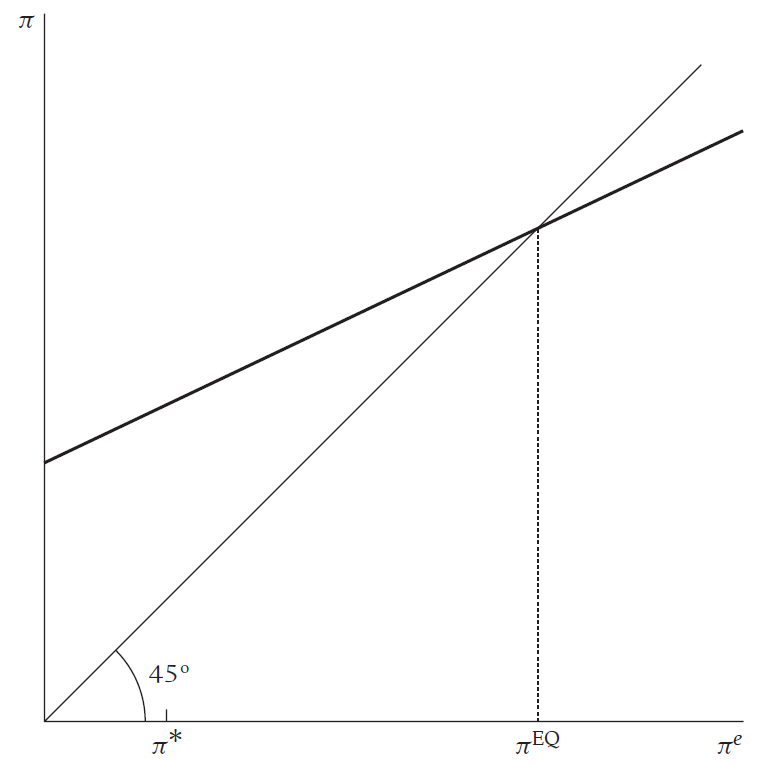
\includegraphics[width=0.6\textwidth]{./figures/aula13_fig1.PNG}
    \caption{Determinação da inflação na ausência de comprometimento. Fonte: Romer (2018).}
    \label{fig1}
\end{figure}

A Figura \ref{fig1} mostra a escolha de $\pi$ pela autoridade monetária como uma função de $\pi^e$. A curva é positivamente inclinada, com uma inclinação menor que 1. A figura e a equação de determinação de inflação mostra o incentivo por parte da autoridade monetária para adotar uma política expansionista. Se os agentes esperam que o Banco Central escolha a taxa ótima de inflação, $\pi^*$, então o custo marginal de uma inflação levemente mais elevada é zero e o benefício marginal do produto mais alto resultante é positivo. Portanto, nesta situação, o formulador de política escolhe uma taxa de inflação maior que $\pi^*$.

Como não há incerteza neste modelo, o equilíbrio requer que a expectativa de inflação e a inflação observada sejam iguais. Como evidenciado pela Figura \ref{fig1}, existe uma única taxa de inflação que satisfaz essa condição. Se temos que $\pi = \pi^e$, então:
\begin{eqnarray*}
\pi^e &=& \pi^* + \frac{b}{a}(y^*-y^n) \\
&\equiv& \pi^{EQ}.
\end{eqnarray*}
Se a expectativa de inflação excede este nível, então, a inflação observada é menor que a esperada pelos agentes e, portanto, a economia não está em equilíbrio. De forma similar, se $\pi^e$ é menor que $\pi^{EQ}$, então, $\pi$ excede $\pi^e$.

Portanto, o único equilíbrio é quando $\pi$ e $\pi^e$ são iguais a $\pi^{EQ}$ e, portanto, $y$ se iguala a $y^n$. Em resumo, \textcolor{blue}{tudo que o poder de  discrição da autoridade monetária faz é aumentar a inflação sem afetar o produto agregado}.

\begin{figure}[h!]
    \centering
    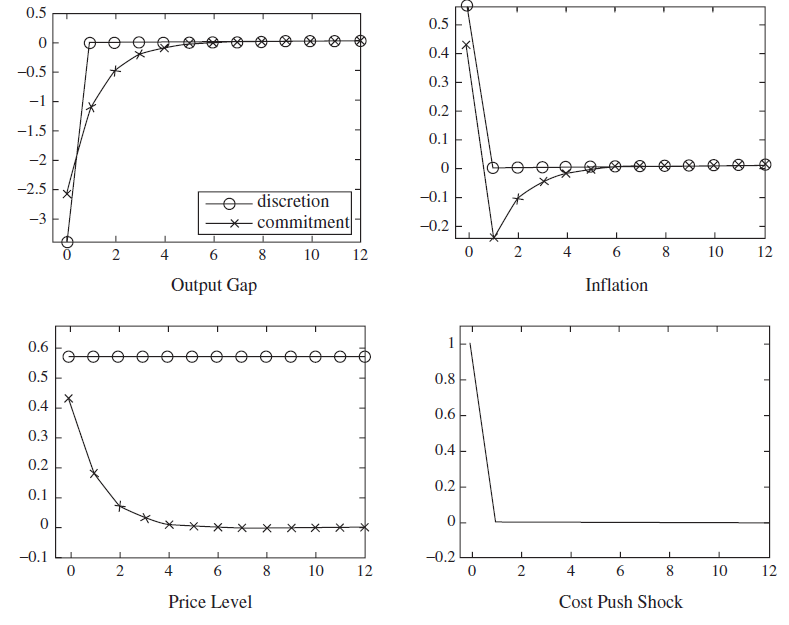
\includegraphics[width=0.8\textwidth]{./figures/aula13_fig2.PNG}
    \caption{Resposta ótima a um choque transitório de oferta. Fonte: Gali (2008).}
    \label{fig:my_label}
\end{figure}

\begin{thebibliography}{}
    \bibitem{gali}
    GALÍ, J. Monetary policy, inflation, and the business cycle: An introduction to the New Keynesian framework. Princeton University Press, 2008.
    
    \bibitem{romer}
    ROMER, D. Advanced Macroeconomics. 5.ed. New York, NY: McGraw-Hill Education, 2018.
    \end{thebibliography}
\end{document}